\documentclass{article}
\usepackage{graphicx,fancyhdr,amsmath,amssymb,amsthm,subfig,url,hyperref}
\usepackage[margin=1in]{geometry}
\usepackage{algorithm, algorithmicx, algpseudocode, graphicx, physics, tikz}
\usepackage{afterpage}

%----------------------- Macros and Definitions --------------------------

\newcommand{\studentname}{Francis Zhang}
\newcommand{\suid}{xz3279}
\newcommand{\exerciseset}{Homework 6}

\renewcommand{\theenumi}{\bf \Alph{enumi}}

\fancypagestyle{plain}{}
\pagestyle{fancy}
\fancyhf{}
\fancyhead[RO,LE]{\sffamily\bfseries\large Columbia University}
\fancyhead[LO,RE]{\sffamily\bfseries\large CSORE 4231 ANALYSIS OF ALGORITHMS I}
\fancyfoot[LO,RE]{\sffamily\bfseries\large \studentname:  \suid}
\fancyfoot[RO,LE]{\sffamily\bfseries\thepage}
\renewcommand{\headrulewidth}{1pt}
\renewcommand{\footrulewidth}{1pt}

\graphicspath{{figures/}}

%-------------------------------- Title ----------------------------------

\title{CSORE 4231 ANALYSIS OF ALGORITHMS I \exerciseset}
\author{\studentname  \qquad \suid}

%--------------------------------- Text ----------------------------------

\begin{document}
\maketitle

\section*{1. Minimum-cost circulation}
Solution:
\begin{enumerate}
    \item[a.] 
    \begin{alignat*}{2}
    \text{maximize}   \quad & \sum_{(u,v) \in E} a(u, v)f_{uv} \\
    \text{subject to} \quad & f_{uv} \leq c(u, v) &\quad& \text{for each } u, v \in V,\\
                        & \sum_{v \in V} f_{vu} - \sum_{v \in V} f_{uv} = 0 && \text{for each } u, v \in V,\\
                        & f_{uv} \geq 0 && \text{for each } u, v \in V.
    \end{alignat*}
    \item[b.] If \(a(u,v) > 0\) for every pair of vertices, then, there is no point in sending any flow at all. So, an optimal solution is just to have no flow. This obviously satisfies the capacity constraints, it also satisfies the conservation constraints because the flow into and out of each vertex is zero.
    \item[c.] We assume that the edge \((t, s)\) is not in \(E\) because that would be a silly edge to have for a maximum flow from \(s\) to \(t\). If it is there, remove it and it won't decrease the maximum flow. Let \(V' = V\) and \(E' = E \cup \{(t, s)\}\). For the edges of \(E'\) that are in \(E\), let the capacity be as it is in \(E\) and let the cost be 0. For the other edge, we set \(c(t, s) = \infty\) and \(a(t, s) = -1\). Then, if we have any circulation in \(G'\), it will be trying to get as much flow to go across the edge \((t, s)\) in order to drive the objective function lower, the other flows will have no effect on the objective function. Then, by Kirchhoff’s current law, the amount going across the edge \((t, s)\) is the same as the total flow in the rest of the network from \(s\) to \(t\). This means that maximizing the flow across the edge \((t, s)\) is also maximizing the flow from \(s\) to \(t\). So, all we need to do to recover the maximum flow for the original network is to keep the same flow values, but put away the edge \((t, s)\).

    \item[d.] Suppose that \( s \) is the vertex that we are computing shortest distance from. Then, we make the circulation network by first starting with the original graph, giving each edge a cost of whatever it was before and infinite capacity. Then, we place an edge going from every vertex that is not \( s \) to \( s \) that has a capacity of 1 and a cost of \( -|E| \) times the largest cost appearing among all the edge costs already in the graph. Giving it such a negative cost ensures that placing other flow through the network in order to get a unit of flow across it will cause the total cost to decrease. Then, to recover the shortest path for any vertex, start at that vertex and then go to any vertex that is sending a unit of flow to it. Repeat this until reached \( s \).
\end{enumerate}

\section*{2. Integer linear programming}
Solution:\\
First, I would like to show this problem is in NP. Let the certificate be vector \(\mathbf{x}\). \(\mathbf{A}\mathbf{x}\) can be computed in \(O(nm)\). Finally, element-wise comparison of \(\mathbf{A}\mathbf{x}\) and \(\mathbf{b}\) can be performed in \(O(m)\) to determine if \(\mathbf{A}\mathbf{x} \leq \mathbf{b}\). This proves a certificate for the problem can be verified in polynomial time.\\
Next, I'm going to show that every problem from the class NP can be reduced to SAT. Consider a system of linear inequalities \( \mathbf{A}\mathbf{x} \geq \mathbf{b} \), where

\[
\mathbf{A} = \begin{bmatrix}
a_{11} & a_{12} & \cdots & a_{1n} \\
a_{21} & a_{22} & \cdots & a_{2n} \\
\vdots & \vdots & \ddots & \vdots \\
a_{m1} & a_{m2} & \cdots & a_{mn}
\end{bmatrix}, \quad
\mathbf{x} = \begin{bmatrix}
x_1 \\
x_2 \\
\vdots \\
x_n
\end{bmatrix}, \quad
\mathbf{b} = \begin{bmatrix}
b_1 \\
b_2 \\
\vdots \\
b_m
\end{bmatrix}.
\]\\
The inequalities are:
\[
\begin{aligned}
a_{11}x_1 + a_{12}x_2 + \cdots + a_{1n}x_n &\geq b_1 \\
a_{21}x_1 + a_{22}x_2 + \cdots + a_{2n}x_n &\geq b_2 \\
\vdots \quad & \quad \vdots \\
a_{m1}x_1 + a_{m2}x_2 + \cdots + a_{mn}x_n &\geq b_m \\
\end{aligned}
\]
For each equation $\sum_{j=i}^{n} a_{ij}x_j \geq b_i$, we can set it as $f_{i1}(x_1) \lor f_{i2}(x_2) \lor \ldots f_{in}(x_n)$. Where $f$ is defined as:
$\begin{array}{l} 
  f_{ij}(x)=\left\{\begin{matrix} 
  x \text{ the representing $a_{ij}$ is positive} \\ 
  0 \text{ the representing $a_{ij}$ is zero} \\ 
  \lnot x \text{ the representing $a_{ij}$ is negative} 
\end{matrix}\right.    
\end{array}$
\\
And we use $\land$ to connect every $f_{i1}(x_1) \lor f_{i2}(x_2) \lor \ldots f_{in}(x_n)$. We now have a SAT problem. So, that SAT is NP-complete.\\
We can convert it to a 3-SAT problem in polynomial time.(For instance, we have a SAT problem $C_i=x_a^i \lor x_b^i \lor x_c^i\lor x_d^i$. We can convert it to $(x_a^i \lor x_b^i \lor w^i)\land(\lnot w^i \lor x_c^i\lor x_d^i)$ where $w^i$ is a fresh variable.) So, SAT can be reduced to 3-SAT. For the SAT $C=C_1 \land \ldots \land C_n$, if we can find out a solution to have $C=1$, we can have a solution to the 3-SAT. Hence, every problem from the class NP can be reduced to 3-SAT, which indicates this 0-1 integer programming is NP-complete.

\section*{3. Bonnie and Clyde}
Solution:
\begin{enumerate}
    \item[a.] We can solve this problem in polynomial time as follows. Let \( a \) denote the number of coins of denomination \( x \) and \( b \) denote the number of coins of denomination \( y \). Then we must have \( a + b = n \). In order to divide the money exactly evenly, we need to know if there is a way to make \( (ax + by)/2 \) out of the coins. In other words, we need to determine whether there exist nonnegative integers \( c \) and \( d \) less than or equal to \( a \) and \( b \) respectively such that \( cx + dy = (ax + by)/2 \). There are \( (a + 1)(b + 1) \leq (n + 1)^2 \) many such linear combinations. We can compute each one in time polynomial in the length of the input numbers, and there are polynomially many combinations to compute, so we can just check all combinations to see if we find one that works.
    \item[b.] We can solve this problem in polynomial time as follows. Start by arranging the coins from largest to smallest. If there are an even number of the current largest coin, distribute them evenly to Bonnie and Clyde. Otherwise, give the extra one to Bonnie and then only give coins to Clyde until the difference has been resolved. This clearly runs in polynomial time, so we just need to show that this will always yield an even division if such a division is possible. Suppose that for some input of coins which can be divided evenly, the algorithm fails. Then there must exist a last time at which there were an odd number of a denomination \(2^i\), so that Bonnie got ahead and had \(2^i\) more dollars than Clyde. At this point, we start giving coins only to Clyde. Since every denomination decrease cuts the amount in half, it will never be the case that Clyde had strictly less than Bonnie, was given an additional coin, and then had an amount strictly greater than Bonnie. Thus, the sum of all coins of size less than \(2^i\) must not exceed \(2^i\). Since we assumed the coins can be divided evenly, there exists \(b_0, b_1, \ldots\) and \(c_0, c_1, \ldots\) such that we assign Bonnie \(b_i\) coins of value \(2^i\) and Clyde \(c_i\) coins of value \(2^i\), and both receive an equal amount. Now remove all coins of value smaller than \(2^i\). Bonnie now has \(\sum_{k=i}^{\infty} b_k 2^k\) dollars and Clyde has \(\sum_{k=i}^{\infty} c_k 2^k\) dollars. Moreover, we know that there is an uneven distribution of wealth at this point, and since every coin has value at least \(2^i\), the difference is at least \(2^i\). Since the sum of the smaller coins is strictly less than \(2^i\), there is no way to distribute the smaller coins to fix the difference, a contradiction since we started with an even split. Thus, the proposed algorithm is correct.
    \item[c.] This problem is NP-complete. First, an assignment of each check to either Bonnie or Clyde represents a certificate which can be checked in polynomial time by adding up the amounts on each of Bonnie's checks, and ensuring that it is equal to the sum of the amounts on each of Clyde’s checks. Next, we'll show this problem, SPLIT-CHECKS is NP-hard by showing that SET-PARTITION \(\leq_p\) SPLIT-CHECKS. Let \( S \) be a set of numbers. We can think of each one as giving the value of a check. If there exists a set \( A \subseteq S \) such that \( \sum_{x \in A} x = \sum_{x \in (S - A)} x \), then we can assign each check in \( A \) to Bonnie and each check in \( S - A \) to Clyde to get an equal division. On the other hand, if there is a way to evenly assign checks then we may just take \( A \) to be the set of checks given to Bonnie, so by contrapositive, if we can’t find a set partition which evenly splits the set then we can’t evenly divide the checks. Thus, the problem is NP-hard, so it is NP-complete.
    \item[d.] An assignment of each check to either Bonnie or Clyde represents a certificate, and we can check in polynomial time whether or not the total amounts given to Bonnie and Clyde differ by at most 100. Thus, the problem is in NP. Next, we'll show it’s NP-hard by showing SET-PARTITION \(\leq_p\) SPLIT-CHECKS-100. Let \( S = \{s_1, s_2, \ldots, s_n\} \) be a set, and let \( xS = \{xs_1, xs_2, \ldots, xs_n\} \). Choose \( x = \min_{i,j} \frac{s_i - s_j}{101} \). Then the difference between any two elements in \( xS \) is more than 100. If there exists \( A \subseteq S \) such that \( \sum_{s \in A} s = \sum_{s \in (S - A)} s \), then we give Bonnie all the checks in \( xA \) and Clyde all the checks in \( x(S - A) \), for a perfectly even split of the money, which means the difference is less than 100. On the other hand, suppose there exists no such \( A \). Then for any way of splitting the elements of \( S \) into two sets, their sums will differ by at least the minimum difference of elements in \( S \). Thus, any way of splitting the checks in \( xS \) will result in a difference of at least 101, so there is no way to split them so that the difference is at most 100. Therefore SET-PARTITION \(\leq_p\) SPLIT-CHECKS-100, so the problem is NP-hard. Since we showed it is in NP, it is also NP-complete.

\end{enumerate}

\section*{4. Vertex Cover approximation}
Solution:\\
Counterexample: Initially, we will choose the central vertex to cover $C$ and delete it from the graph. After that we will choose the other vertices randomly until the graph is empty. This result is greater than two times optimal solution.\\
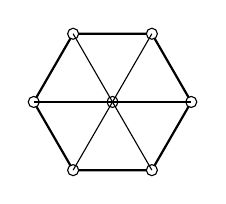
\begin{tikzpicture}
% 定义六边形的中心
\coordinate (center) at (0,0);

% 绘制六边形并在每个顶点放置一个圆圈
\draw[thick] (0:1) -- (60:1) -- (120:1) -- (180:1) -- (240:1) -- (300:1) -- cycle;
\foreach \angle in {0, 60, 120, 180, 240, 300} {
    \filldraw[fill=white, draw=black] (\angle:1) circle (2pt);
    \coordinate (vertex\angle) at (\angle:1);
}

% 在中心添加一个圆圈
\filldraw[fill=white, draw=black] (center) circle (2pt);

% 将中心与六个顶点连接
\foreach \angle in {0, 60, 120, 180, 240, 300} {
    \draw[thin] (center) -- (vertex\angle);
}

\end{tikzpicture}

\end{document}
